\sectioncounter{14}
  \section{利用导数研究函数的最(极)值}

  \subsection{知识梳理}
  若函数 $f(x)$ 在点 $x=x_0$ 左侧递增而在其右侧递减, 则称 $f(x_0)$ 为 $f(x)$ 的极大值; 
  若 $f(x)$ 在点 $x=x_0$ 左侧递减而在其右侧递增, 则称 $f(x_0)$ 为 $f(x)$ 的极小值. 
  在两种情况下, 都称点 $x_0$ 为 $f(x)$ 的极值点, $f(x_0)$ 为 $f(x)$ 的极值,
  参见下面的表格. 注意, 函数的极大值可能小于极小值.
  由导数的正负号与函数增减性之间的关系可知, 极值点 $x_0$ 处左右侧导数值异号, 
  所以必有 $f'(x_0)= 0$, 即函数的极值点是其导数的零点. 
  但是导数的零点不一定是函数的极值点 (考虑 $y=x^3$ 在点 $x=0$ 附近的图象), 还需确定附近的导数正负号再由定义判断.
  \begin{center}
    \small
    \begin{tabular}{c|ccc}
         $x$  & 左侧 & $x_0$ & 右侧 \\
      \hline
      $f'(x)$ & $-$ & 0 & $+$ \\
      $f(x)$ & $\searrow$ & 极小值 & $\nearrow$
    \end{tabular}
    \qquad
    \begin{tabular}{c|ccc}
        $x$   & 左侧 & $x_0$ & 右侧 \\
      \hline
      $f'(x)$ & $+$ & 0 & $-$ \\
      $f(x)$ & $\nearrow$ & 极大值 & $\searrow$
    \end{tabular}
  \end{center}
  
  函数的最值指其最大值和最小值. 由函数图象可以知道, 最值若存在, 
  则一定在极值或端点值中取到. 所以求函数的最值, 应先求出所有极值和端点值, 再作比较.
  最值不一定是极值, 极值也不一定是最值, 需借助图象具体判断.

  \lianxi
  \begin{exercise}
    求函数 $y=x^3 -3x+9$ 的极小值.
  \end{exercise}

  \beginsolution
    $y'=3(x+1)(x-1)$, 则 $x=1$ 时, $y=7$ 为极小值.
  \endsolution

  \begin{exercise}
    求函数 $y=\frac{\ln x}x$ 的最值.
  \end{exercise}

  \beginsolution
    $y'=\frac{1-\ln x}{x^2}$, 则 $x=\mathrm{e}$ 时, $y=\frac1{\mathrm{e}}$ 为最大值, 无最小值.
  \endsolution
  
  \begin{exercise}
    函数 $f(x)=x^3 +3x^2 +4x-a$ 的极值点有多少个\,?
  \end{exercise}

  \beginsolution
    $f'(x)=3x^2+6x+4=3(x+1)^2+1>0$, 则 $f(x)$ 在 $\mathbb{R}$ 上 $\nearrow$, 无极值点.
  \endsolution
  
  \begin{exercise}
    若 $y=2x^3 -3x^2 -12x+a$ 在 $D=[0,2]$ 上的最大值为 $5$, 求 $a$ 的值.
  \end{exercise}

  \beginsolution
    $y'=6(x+1)(x-2)$, 则 $y$ 在 $[0,2]$ 上 $\searrow$, 当 $x=0$ 时, $y=a$ 为最大值, 所以 $a=5$.
    
    \varexercise 若 $D=[2,4]$, 其余条件不变, 求 $a$ 的值.
    
    由 $y'=6(x+1)(x-2)$ 知 $y$ 在 $[2,4]$ 上 $\nearrow$, 当 $x=4$ 时, $y=32+a$ 为最大值, 所以 $a=-27$.
    
    \varexercise 若 $D=[1,3]$, 其余条件不变, 求 $a$ 的值.
    
    由 $y'=6(x+1)(x-2)$ 知 $y$ 在 $[1,2)$ 上 $\searrow$, 在 $(2,3]$ 上 $\nearrow$. 而当 $x=1$ 时, $y=a-13$, 当 $x=3$ 时, $y=a-9$, 所以 $a-9$ 为最大值, $a=14$.
  \endsolution
  
  \subsection{要点导学\quad 各个击破}
  \subsubsection{利用导数研究函数的极值}
  \begin{example}
    求下列函数的极值:
    
    (1) $f(x)=2x^3 -6x^2 +1$;\qquad
    (2) $f(x)=\frac{\ln x}{x^2}$.
  \end{example}

  \beginsolution
    (1) $f'(x)=6x(x-2)$, 则极大值为 $f(0)=1$, 极小值为 $f(2)=-7$.
    
    (2) $f'(x)=\frac{1-2\ln x}{x^3}$, 
    \mymarginpar{结论一般化: $f(x)=\frac{\ln x}{x^n}$ ($n$ 为正整数) 的最大值为 $f(\sqrt[n]{\mathrm{e}})=\frac1{n\mathrm{e}}$.}
    则极大值 (也是最大值) 为 $f(\sqrt{\mathrm{e}})=\frac1{2\mathrm{e}}$, 无极小值.
  \endsolution
  
  \begin{example}
    已知函数 $f(x)=x^3 -3x+a$ 
    
    (1) 若 $f(x)$ 恰有两个零点, 求 $a$ 的值;
    
    (2) 若 $f(x)$ 有三个零点,求 $a$ 的取值范围.
  \end{example}

  \beginsolution
    $f'(x)=3(x+1)(x-1)$, 
  \mymarginpar{函数 $f(x)$ 的图象:
    \begin{center}
    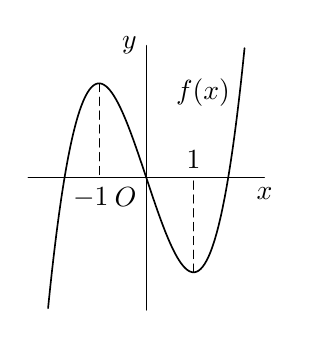
\begin{tikzpicture}[line cap=round,line join=round,scale=0.6]
      \draw[\myaxisarrow] (-2.5,0) -- (2.5,0) node[below] {$x$};
      \draw[\myaxisarrow] (0,-2.8) -- (0,2.8) node[left] {$y$};
      \draw[line width=0.6pt,smooth,samples=100] 
        plot[domain=-2.08:2.08](\x,{(\x)^3-3*\x});
      \draw[densely dashed] (-1,2)--(-1,0) node[below,xshift=-3pt] {$-1$}
        (1,-2)--(1,0) node[above] {$1$};
      \draw (0,0) node[anchor=north east] {$O$}
        (1.2,1.8) node {$f(x)$};
    \end{tikzpicture}\end{center}}
    讨论 $f(x)$ 的单调性可知大致图象如右图 (可上下平移).
    
    (1) 此时 $f(-1)=0$ 或 $f(1)=0$, 则 $a=-2$ 或 $2$.
    
    (2) 此时 $f(-1)>0$ 且 $f(1)<0$, 则 $-2<a<2$.
  \endsolution
  
  \lianxi
  \begin{exercise}[s]
    已知函数 $f(x)=\dfrac13 x^3 +a^2 x^2 +ax+b$, 当 $x=-1$ 时, 
    $f(x)$ 的极值为 $-\dfrac7{12}$, 求 $f(2)$ 的值.
  \end{exercise}

  \beginsolution
    $f'(x)=x^2+2a^2x+a$, 由题意, $f'(-1)=0$, 
    \mymarginpar{$f'(x_0)=0$ 只是 $f(x_0)$ 为极值的必要条件, 解得的参数值必须检验.}
    则 $a=1$ 或 $-\frac12$. 而当 $a=1$ 时, 
    \[f'(x)=(x+1)^2\geqslant 0,\]
    $f(x)$ 无极值; 当 $a=-\frac12$ 时, 
    \[f'(x)=(x+1)\Bigl(x-\frac12\Bigr),\]
    $f(-1)$ 为极大值, 故 $a=-\frac12$. 由 $f(-1)=-\frac7{12}$ 知 $b=0$, 所以 $f(2)=\frac83$.
  \endsolution
  
  \subsubsection{利用导数研究函数的最值}
  \begin{example}
    已知 $f(x)=ax- \dfrac2x -3\ln x$, 其中 $a$ 为常数.
    若函数 $f(x)$ 的图象在点 $\Big(\dfrac23, f\Big(\dfrac23\Big)\Big)$ 
    处的切线的斜率为 $1$, 求 $f(x)$ 在 $\Big[\dfrac32,3\Big]$ 上的最小值.
  \end{example}

  \beginsolution
    $f'(x)=a+\frac2{x^2}-\frac3x$. 由 $f'\Bigl(\frac23\Bigr)=1$ 知 $a=1$, 所以 
    \[f'(x)=\frac{(x-1)(x-2)}{x^2},\]
    表明 $f(x)$ 在 $\Big[\dfrac32,3\Big]$ 上的最小值为 $f(2)$. 而 $f(x)=x-\frac3x-3\ln x$, 所以 $f(2)=1-3\ln2$.
  \endsolution
  
  \lianxi
  \begin{exercise}
    已知函数 $f(x)=\ln x+ \frac2{x^2}$, 求 $f(x)$ 的最小值.
  \end{exercise}

  \beginsolution
    $f'(x)=\frac{(x+2)(x-2)}{x^3}$, 由 $x>0$ 知 $f(x)$ 在 $(0,2)$ 上 $\searrow$, 在 $(2,+\infty)$ 上 $\nearrow$, 故最小值为 $f(2)=\ln 2+\frac12$.
  \endsolution
  
  \begin{exercise}
    若 $f(x)=(x-a)\ln x$ 的导数 $f'(x)=\ln x+1$, 求 $f(x)$ 的最小值.
  \end{exercise}

  \beginsolution
    由 $f'(x)=\ln x+\frac{x-a}x= \ln x+1$ 知 $a=0$, 且 $f(x)$ 在 $\Big(0,\frac1{\mathrm{e}}\Big)$ 上 $\searrow$, 在 $\Big(\frac1{\mathrm{e}},+\infty\Big)$ 上 $\nearrow$, 则最小值为 $f\Big(\frac1{\mathrm{e}}\Big)$. 由 $f(x)=x\ln x$ 知 $f\Big(\frac1{\mathrm{e}}\Big)=-\frac1{\mathrm{e}}$.
  \endsolution
  
  \subsubsection{恒成立问题}
  \begin{example}
    已知函数 $f(x)=\mathrm{e}^x -kx$, $x\in\mathbb{R}$.
    
    (1) 若 $k=\mathrm{e}$, 求函数 $f(x)$ 的单调区间;
    
    (2) 若 $k>0$ 且 $f(x)>0$ 在 $(0,+\infty)$ 上恒成立, 求 $k$ 的取值范围.
  \end{example}

  \beginsolution
    $f'(x)=\mathrm{e}^x-k$.
    
    (1) 此时 $f'(x)=\mathrm{e}^x-\mathrm{e}$, 则 $f(x)$ 在 $(-\infty,1)$ 上 $\searrow$, 在 $(1,+\infty)$ 上 $\nearrow$.
    
    (2) 方法一: 若 $0<k\leqslant 1$, 则在 $(0,+\infty)$ 上, $f'(x)\geqslant f'(0)\geqslant 0$, 表明 $f(x)\nearrow$.
    
    若 $k>1$, 则 $f(x)$ 在 $(0,\ln k)$ 上 $\searrow$, 在 $(\ln k,+\infty)$ 上 $\nearrow$, 只需 $f(\ln k)>0$, 解得 $k<\mathrm{e}$.
    
    综上所述, $k\in(0,\mathrm{e})$.
    
    方法二: $f(x)>0$ 化为 $k<\frac{\mathrm{e}^x}x$. 
    \mymarginpar{用分离常数法 (方法二) 显得更直接, 且容易看出在题中无需限制 $k>0$.}
    设 $g(x)=\frac{\mathrm{e}^x}x$, $x\in(0,+\infty)$, 则 $g'(x)=\frac{\mathrm{e}^x (x-1)}{x^2}$, 表明 $g(x)$ 在 $(0,1)$ 上 $\searrow$, 在 $(1,+\infty)$ 上 $\nearrow$. 所以 $k<g_{\min}=g(1)=\mathrm{e}$.
  \endsolution
  
  \begin{example}
    若函数 $f(x)=x^3-ax+2$ 在 $[1,+\infty)$ 上恒正, 求 $a$ 的取值范围.
  \end{example}

  \beginsolution
    $f(x)>0$ 化为 $x^2+\frac2x>a$. 
    \mymarginpar{此例也可以直接讨论 $f(x)$ 的单调性, 但是要根据 $a$ 的取值分为多种情况 (如何分类\,?). 一般先考虑用分离参数法.}
    设 $g(x)=x^2+\frac2x$, $x\in[1,+\infty)$, 则 $g'(x)=\frac{2(x^3-1)}{x^2}$, 表明 $g(x)$ 在 $[1,+\infty)$ 上 $\nearrow$, 所以 $a<g_{\min}=g(1)=3$.
  \endsolution
  
  \subsubsection{课堂评价}
  \begin{exercise}
    求函数 $f(x)=x^3 -3x+1$ 在 $[0,2]$ 上的最大值.
  \end{exercise}

  \beginsolution
    $f'(x)=3(x+1)(x-1)$, 表明 $f(x)$ 在 $[0,1)$ 上 $\searrow$, 在 $(1,2]$ 上 $\nearrow$, 则最大值为 $\max\{f(0),f(2)\}=3$.
  \endsolution
  
  \begin{exercise}
    设函数 $f(x)=x^2-2x-4\ln x$, 求其最值.
  \end{exercise}

  \beginsolution
    $f'(x)=\frac{2(x+1)(x-2)}x$ 且 $x>0$, 表明 $f(x)$ 在 $(0,2)$ 上 $\searrow$, 在 $(2,+\infty)$ 上 $\nearrow$, 最小值为 $f(2)=-4\ln 2$, 无最大值.
  \endsolution
  
  \begin{exercise}
    若函数 $f(x)=x(\ln x-ax)$ 有两个极值点, 求 $a$ 的取值范围.
  \end{exercise}

  \beginsolution
    $f'(x)=\ln x-2ax+1$ 有两个零点.
    
    方法一: 由  $f''(x)=\frac1x-2a$ 和 $x>0$ 知  $a>0$ (否则 $a\leqslant 0$ 时, $f''(x)\geqslant 0$, 表明 $f'(x)$ 在 $(0,+\infty)$ 上 $\nearrow$, 至多一个零点). 所以 $f'(x)$ 在 $\Big(0,\frac1{2a}\Big)$ 上 $\nearrow$, 在 $\Big(\frac1{2a},+\infty\Big)$ 上 $\searrow$, 
    \mymarginpar{当 $\alpha>0$, $x$ 充分大时, 
      \[x^\alpha\gg \ln x,\quad \text{或}\quad \alpha x\gg \ln x.\]}
    由 $f'(0)=-\infty$, $f'(+\infty)=-\infty$ 知, 只需 $f'\Big(\frac1{2a}\Big)>0$, 即 $0<a<\frac12$.
    
    方法二: $2a=\frac{1+\ln x}x$ 有两个零点, 设 $g(x)=\frac{1+\ln x}x$, $x>0$, 则 $g'(x)=-\frac{\ln x}{x^2}$, 表明 $g(x)$ 在 $(0,1)$ 上 $\nearrow$, 在 $(1,+\infty)$ 上 $\searrow$, 所以 $g(x)$ 最大值为 $g(1)=1$, 而 $g(0)=-\infty$, $g(+\infty)=0$, 故由 $g(x)$ 的图象, $2a\in(0,1)$, 即 $a\in\Big(0,\frac12\Big)$.
  \endsolution
  
  \subsection{课后练习}
  \begin{exercise}
    求函数 $f(x)=x-\mathrm{e}^x$ 在 $[0,1]$ 上的最小值.
  \end{exercise}

  \beginsolution
    $f'(x)=1-\mathrm{e}^x$ 在 $(0,1]$ 上小于 $0$, 故 $f(x)$ 在 $[0,1]$ 上 $\searrow$, 最小值为 $f(1)=1-\mathrm{e}$.
  \endsolution
  
  \begin{exercise}
    求函数 $f(x)=x+2\cos x$ 在 $\Big[0,\frac{\pi}2\Big]$ 的最大值.
  \end{exercise}

  \beginsolution
    $f'(x)=1-2\sin x$, 表明 $f(x)$ 在 $\Big[0,\frac\pi6\Big)$ 上 $\nearrow$, 在 $\Big(\frac\pi6,\frac{\pi}2\Big]$ 上 $\searrow$, 最大值为 $f\Big(\frac\pi6\Big)= \frac\pi6+\sqrt3$.
  \endsolution
  
  \begin{exercise}
    若函数 $f(x)=\mathrm{e}^x\sin x$, $x\in[0,\pi]$, 求其最值.
  \end{exercise}

  \beginsolution
    $f'(x)=(\sin x+\cos x)\mathrm{e}^x$, 表明 $f(x)$ 在 $\Big[0,\frac{3\pi}4\Big)$ 上 $\nearrow$, 在 $\Big(\frac{3\pi}4,\pi\Big]$ 上 $\searrow$, 最大值为 $f\Big(\frac{3\pi}4\Big)= \frac{\sqrt2}2\mathrm{e}^{\frac{3\pi}4}$, 最小值为 $\min\{f(0),f(\pi)\}=0$.
  \endsolution
  
  \begin{exercise}
    若函数 $f(x)=x^3 +ax^2 +ax$ ($x\in\mathbb{R}$) 无极值点,
    求 $a$ 的取值范围.
  \end{exercise}

  \beginsolution
    $f'(x)=3x^2+2ax+a$ 不变号, 故 $(2a)^2-4\cdot 3\cdot a\leqslant 0$,  $a\in[0,3]$.
  \endsolution
  
  \begin{exercise}
    已知函数 $f(x)=x^3 +ax^2 +3x-9$ 在 $x=-3$ 时取得极值, 求 $a$ 的值.
  \end{exercise}

  \beginsolution
    $f'(x)=3x^2+2ax+3$ 且 $f(-3)=0$, 
    \mymarginpar{一定要检验 $a$ 是否使得 $x=-3$ 为极大值点.}
    则 $a=5$, 此时 $f'(x)=(x+3)(3x+1)$, $x=-3$ 为极大值点.
  \endsolution
  
  \begin{exercise}
    已知函数 $f(x)=\mathrm{e}^x (ax+b)-x^2 -4x$, 曲线 $y=f(x)$ 
    在点 $(0,f(0))$ 处的切线方程为 $y=4x+4$. 讨论 $f(x)$ 的单调性,
    并求其极大值.
  \end{exercise}

  \beginsolution
    $f'(x)=\mathrm{e}^x(ax+a+b)-2x-4$, 则
    \[\left\{\!\!\begin{array}{l}
      f'(0)= a+b-4=4,\\
      f(0)= b=4,\end{array}\right.\]
    即 $a=b=4$, 
    \[f'(x)=2(2\mathrm{e}^x-1)(x+2),\] 表明 $f(x)$ 在 $(-\infty,-2)$ 和 $(-\ln2,+\infty)$ 上 $\nearrow$, 在 $(-2,-\ln2)$ 上 $\searrow$, 极大值为 $f(-2)$. 由 $f(x)=4\mathrm{e}^x(x+1)-x^2-4x$ 知, $f(-2)=4(1-\mathrm{e}^x)$.
  \endsolution

  \begin{exercise}
    若 $x\ln x\geqslant -x^2+ax-6$ 在 $(0,+\infty)$ 上恒成立, 求 $a$ 的取值范围.
  \end{exercise}

  \beginsolution
    不等式化为 $a\leqslant x+\frac6x+\ln x$, 
    \mymarginpar{此题无法直接讨论不等式两边作差后得到式子的单调性.}
    设 $f(x)=x+\frac6x+\ln x$, $x>0$, 则 
    \[f'(x)=\frac{(x-2)(x+3)}x,\]
    表明 $f(x)$ 在 $(0,2)$ 上 $\searrow$, 在 $(2,+\infty)$ 上 $\nearrow$, 所以 $f_{\min}=f(2)=5+\ln 2$, 故 $a\in(-\infty,5+\ln2]$.
  \endsolution
%%%%%%%%%%%%%%%%%%%%%%%%%%%%%%%%%%%%%%%%%%